\cotefile{79}
\scanpage{97}
\mspage{48}

Je peux reprendre maintenant le fil des réflexions du § III. Soit

\[
\Lambda=\mathbb Z/n\mathbb Z\qquad\text{avec }n\in\mathbb N^{*},\ n\ne 2,4
\]

et considérons un module libre de rg $2$ $M$ sur $\Lambda$, considérons une des structures $P_{i_0}=P_{M,i_0}$ sur $S_M=S$ $(i_0\in\Pi_M)$ -- alors le groupe des automorphismes $G=G_M$ de $P_{\deleted{\unsure{M}},i_0}$ (en tant que ss-groupe de $\unsure{\mathfrak S|\mathfrak G}_S$) ne dépend pas du choix de $i$, ni d'ailleurs le sous-groupe $G^+$ des autom. directs. Soit $\deleted{\Lambda} Z^{\deleted{\unsure{*|+}}}$ son commutant

\[
\left\{\begin{aligned}
 Z^{\deleted{*}}&=\operatorname{Comm.}_{\mathfrak S_S}(G^+)\\
 G&=\operatorname{Aut}(P_{i_0})\qquad\text{(indépend\unsure{${}^{\rm mt}$|amment|ant} du choix de }i_0\in\Pi\text{)}
\end{aligned}\right. \tag*{(56)}
\]

On a alors

\[
\left\{\begin{aligned}
 &\forall s,t\in S,\ \deleted{\unsure{g}}\lambda\in Z,\ \deleted{\unsure{i\in\Pi},}\ \text{on a}\\
 &\{s,t\}\in A_{i_0}\iff \{\lambda s,\lambda^{-1}t\}\in A_{i_0}\implies t\ne\lambda.s
\end{aligned}\right. \tag*{(57)}
\]

et de plus

\[
\left\{\begin{aligned}
 &\inserted{\forall\lambda\in Z}\\
 &\text{L'unique structure 2-polyèdre triangulée}\\
 &\text{sur }S,\ \deleted{\text{\unsure{défini}}}\ \deleted{\text{\unsure{comme}}}\ \text{l'ens. d'arêtes }A_\lambda\\
 &\text{défini par}\\
 &\{s',t'\}\in A_\lambda\iff\{s',\lambda^{-1}.t'\}\in A_{i_0}\\
 &\text{est }\deleted{\text{\unsure{donc}}}\ \text{un des }A_i\ (i\in\Pi),\ \text{soit }A_{\lambda.i_0}
\end{aligned}\right. \tag*{(58)}
\]

et enfin
% archive sheet number: 96
\scanpage{98}

\[
\begin{aligned}
 &\text{L'application }\quad\lambda\longmapsto\lambda.i_0\qquad Z\longrightarrow\Pi\\
 &\text{est bijective ; plus précisément,}\\
 &\text{si on considère de \unsure{$\simeq$|$=$} l'application}\\
 &\lambda\longmapsto\lambda.i,\ \text{pour tt choix de }i\in\Pi,\\
 &\text{on trouve que l'ens des structures}\\
 &\text{2-polyédrales }\Pi\text{ sur }S\text{ est un torseur}\\
 &\text{sous }Z.
\end{aligned}\tag*{(59)}
\]

Il faudrait maintenant expliciter l'iso

\[
Z\simeq Z'_\Lambda\simeq\Lambda^*/\{\pm 1_\Lambda\}\tag*{(60)}
\]

en termes de la seule structure combinatoire d'un des $P_i$, soit $P_{i_0}$. Regardons pour ceci, pour $\lambda\in Z$ fixé, et $s\in S$ fixé, l'application

\[
\left\{\begin{aligned}
 \operatorname{Et}_{P_{i_0}}(s)&\overset{\sim}{\longrightarrow}\operatorname{Et}_{P_{\underbrace{\lambda.i_0}_{i_1}}}(s)\\
 t&\longmapsto\lambda.t
\end{aligned}\right.\tag*{(61)}
\]

Notons que les deux mbres sont des torseurs sous les groupes

\[
\left\{\begin{aligned}
 &\deleted{\unsure{\mathbb Z/n\mathbb Z}}\\
 &\Gamma_{i_0}=\Lambda\wedge_{\mu_2}\mu(i_0)\qquad\text{resp }\Gamma_{i_1}=\Lambda\wedge_{\mu_2}\mu(i_1)\\
 &\text{où }\mu(i)=\text{ens des orientations de }P_i
\end{aligned}\right.\tag*{(62)}
\]
% archive sheet number: 97
\scanpage{99}
\mspage{49}

Ceci posé, je dis que

\[
\begin{aligned}
 &\text{L'application (61) }\quad\operatorname{Et}_{P_{i_0}}(s)\overset{\lambda_s}{\overset{\sim}{\longrightarrow}}\operatorname{Et}_{P_{i_1}}(s)\\
 &\text{définie par }\lambda\text{ est un }\deleted{\text{\unsure{bis}}}\text{isomorphisme}\\
 &\text{de torseurs, pour un isomorphisme}\\
 &\text{des groupes d'opérateurs (uniquement}\\
 &\text{déterminé bien sûr)}\\
 &\deleted{\unsure{\gamma}}\lambda_{\Gamma,s}:\quad\Gamma_{i_0}\overset{\sim}{\underset{\unsure{1}}{\longrightarrow}}\Gamma_{i_1},
\end{aligned}\tag*{(63)}
\]

% slanted
\margin{à \uline{vérifier}}

Quand on a choisi des orientations de $P_{i_0}$ et de $P_{i_1}$, i.e. des origines de $\mu(i_0)$ et $\mu(i_1)$, alors $\lambda_{\Gamma,s}$ s'explicite par un isomorphisme de groupes

\[
\Lambda\overset{\sim}{\longrightarrow}\Lambda
\]

donc par un élément \inserted{$\gamma$} de $\Lambda^*$, \deleted{\unsure{point|pris}}\inserted{quand} on change \deleted{d'orientation}\inserted{d'origine} dans l'un des \deleted{\unsure{ensembles ordonnés}}\inserted{torseurs} $\mu(i_0)$, $\mu(i_1)$, \deleted{\unsure{le}} $\gamma$ est remplacé par $-\gamma$. Ainsi, on peut interpréter $\lambda_{\Gamma,s}$ comme un élément

\[
\lambda_{\Gamma,s}\in\bigl[\underbrace{\Lambda\wedge_{\mu_2}\bigl(\mu(i_0)\wedge\mu(i_1)\bigr)}_{\text{$\Lambda$-module inversible}\quad\Gamma_{i_0i_1}}\bigr]^{*}\tag*{(64)}
\]

ou, je le rappelle, $\unsure{i_1|\mu_1}=\lambda.i_0$.

On a d'autre part une \deleted{application}\inserted{\unsure{isom}} \deleted{canonique} canonique

\[
\begin{aligned}
 \Gamma_{i_0i_1}^{*}/\{\pm1\}&\simeq\Lambda^*/\pm1\\
 \unsure{\xi|\zeta}&\longmapsto \xi^{\unsure{\natural|\sharp|4}}
\end{aligned}\tag*{(65)}
\]
% archive sheet number: 98
\scanpage{100}

d'où enfin une application

\[
\begin{aligned}
 Z&\longrightarrow Z'_\Lambda=\Lambda^*/\{\pm1_\Lambda\}\\
 \lambda&\longmapsto(\lambda_{\Gamma,s})^{\unsure{\natural|\sharp|4}}
\end{aligned}\tag*{(66)}
\]

qui a priori dépend du choix de $i_0\in\Pi$, et de $s\in S$. Mais on trouve

\[
\begin{aligned}
 &\text{L'application précédente est indépendante}\\
 &\text{du choix de }s\in S\text{ et de}\\
 &i_0\in\Pi,\ \text{et c'est un \uline{isomorphisme}}\\
 &\text{de groupes (en fait, c'est l'}\\
 &\text{isomorphisme inverse de l'isomorphisme}\\
 &\text{obtenu p. }47'\text{).}
\end{aligned}\tag*{(67)}
\]

% slanted
\margin{à vérifier}

Ainsi, j'ai explicité, en termes d'une quelconque des structures $P_{M,i}$ -- ou de l'ens. de ces structures, au choix \inserted{ou de la structure $F_M$ \unsure{seulement}} -- l'opération de $Z'_\Lambda$ sur $S$, et par là, l'opération de $Z'_\Lambda$ sur $\Pi$, qui fait de $\Pi$ un $Z'_\Lambda$-torseur.

Explicitons maintenant le $\Lambda^*$-torseur $\vec\Pi^{*}$, on a une bijection canonique

\[
\vec\Pi\simeq\coprod_{i\in\Pi}\bigl[\underbrace{\operatorname{Or}(P_{\deleted{\unsure{M}},i})}_{\deleted{\text{\unsure{ou plutôt ens. des deux orientations de |petit ens. des deux orientations de }P_i}}}=\underbrace{\mu(i)}_{\text{ens des deux or de $P_i$}}\bigr]\tag*{(68)}
\]
% archive sheet number: 99
\scanpage{101}
\mspage{50}

\deleted{\unsure{ce}}\inserted{l'interprétation} qui nous donne aussitôt l'application canonique de degré 2

\[
\begin{aligned}
 \unsure{\vec\Pi|\overline\Pi}&\xrightarrow[\text{degré 2}]{}\Pi\\
 \{i,\underset{\substack{\rotatebox{90}{$\in$}\\\deleted{\unsure{\operatorname{Or}}}\unsure{\mu|\chi}(i)}}e\}&\longmapsto i
\end{aligned}\tag*{(69)}
\]

Il faut \deleted{définir}\inserted{\unsure{définir|décrire} combinatoirement} une opération de $\Lambda^*$ sur $\vec\Pi$, de telle façon que (69) soit compatible avec l'application canonique

\[
\deleted{\unsure{(70)}}\qquad\Lambda^*\longrightarrow Z'_\Lambda=\Lambda^*/\{\pm1_\Lambda\}
\]

Soit donc $(i,e\in\deleted{\operatorname{Or}}\mu(i)\deleted{\unsure{P_{M,i}}})\in\vec\Pi$, $\lambda\in\Lambda^*$, $\unsure{\acute\lambda|\dot\lambda}$ son image ds $Z'_\Lambda$ on veut définir

\[
\left\{\begin{aligned}
 &\lambda(i,e)=\deleted{\unsure{\lambda}}(i',e')\qquad e'\in\operatorname{Or}\deleted{\unsure{P_{M,i'}|P_{i'}}}\mu(i')\\
 &i'=\dot\lambda.i,\quad e'=\mathord{?}
\end{aligned}\right.\tag*{(70)}
\]

\deleted{Or considérons l'application (61) ($s\in S$ choisi)}

\[
\deleted{\operatorname{Et}_{P_{i_0}}(s)\longrightarrow\operatorname{Et}_{P_i}(s)}
\]

\deleted{le choix de $e$ définit une orientation du \unsure{$n$}-polygône $\operatorname{Et}_{P_{i_0}}(s)$, qui devient ainsi un torseur sous $\mathbb Z/n\mathbb Z$ ; pour \deleted{\unsure{tt}}\inserted{le choix d'une} orientation $e'$ de $P_{i'}$, faisant de $\operatorname{Et}_{P_i}$}

Choisissons $s\in S$, alors

\[
\lambda_{\Gamma,s}\in\Lambda\wedge_{\mu_2}(\mu(i)\wedge\mu(i'))\xrightarrow{\text{degré 2}} Z'_\Lambda\text{ --}
\]

est au dessus de $\dot\lambda$ ; pour tout $e'\in\mu(i')$,
% archive sheet number: 100
\scanpage{102}
\mspage{5\deleted{\unsure{1|0}}\unsure{0|1}'}

$\exists!\,\lambda_{e'}\in\Lambda$ tel qu'on ait

\[
\lambda_{\Gamma,s}=\lambda_{e'}\underset{\mu_2}{\wedge}(e\wedge e')\tag*{(71)}
\]

et on a bien sur

\[
\lambda_{\deleted{\unsure{e}}\overline{e'}\deleted{\unsure{e}}}=-\lambda_{e'}\qquad\text{si }\mu(i')=\{e',\overline{e'}\}\tag*{(\unsure{72|71})}
\]

Ainsi, $\{\lambda_{e'},\lambda_{\overline{e'}}\}$ est l'image inverse de $\dot\lambda\in\Lambda^*/\pm1$ dans $\Lambda^*$, et il existe un unique $e'\in\mu(i')$, tel qu'on ait

\[
\lambda=\lambda_{e'}\quad\text{i.e.}\quad\lambda_{\Gamma,s}=\lambda\wedge(e\wedge e')\in\Gamma_{ii'}.\tag*{(73)}
\]

A priori, ce choix de $e'$ dépend de celui de $s\in S$ -- en fait il est indépendant de ce choix. On trouve ainsi l'opération de $\Lambda=\mathbb Z/n\mathbb Z$ sur $\deleted{\mathbb Z}\vec\Pi$, qui fait de $\unsure{\vec\Pi|\overline\Pi|\vec\pi}$ un torseur sous $\Lambda$.

L'application

\[
\tau_F:\underbrace{\vec F}_{\text{\unsure{ou|en} }\vec F_M}\quad\unsure{\flat|\ell}\longrightarrow\vec\Pi\tag*{(74)}
\]

qui relève $\tau:F\longrightarrow\Pi$ est maintenant évidente, car \deleted{\unsure{face}}\deleted{toute} face \inserted{orientée} $f\in\vec F$ définit à la fois un $\tau(f)=i\in\Pi$, et un $e\in\deleted{\unsure{P}}\mu(i)=\operatorname{Or}P_i$ orientation de la structure triangulaire à laquelle appartient cette face.
% archive sheet number: 101
\scanpage{103}

\uline{$\overline{\mathrm{VII}}$}\quad\uline{Structures \unsure{triangulées|triangulaires} congruentielles.}

Une \uline{structure triangulaire} est pour nous un couple

\[
\begin{aligned}
 (S,F)\qquad&S\text{ un ensemble (``\uline{sommets}'')}\\
 &\underset{\text{ens. des \uline{faces}}}{F}\subset\unsure{\mathscr P|\mathcal P|\mathfrak P}_3(S)
\end{aligned}\tag*{(1)}
\]

satisfaisant l'axiome

\[
\deleted{\text{(T1)}}\quad\text{\textcircled{\scriptsize T1}}\qquad\deleted{\unsure{S}}\,S=\bigcup_{f\in F}f
\qquad\underset{\deleted{\text{\unsure{bien|lien}}}}{\text{donc}}\quad S\ne\varnothing\iff F\ne\varnothing.\tag*{(2)}
\]

Les structures qui nous intéressent satisfont à des axiomes supplémentaires, inspirés par le cas des $(S_M,F_M)$ où $M$ est un module libre de rang $2$ sur un $\mathbb Z/n\mathbb Z$, $n\geq3$. Posons déjà

\[
\deleted{\text{\unsure{(T1 bis)}}}\qquad\underset{\substack{\text{ens des}\\\text{\uline{arêtes}}}}{A}=\{a\in\mathscr P_2(S)\mid\exists f\in F,\ f\supset a\},\tag*{(3)}
\]

\deleted{\unsure{on}} demande

\[
\begin{aligned}
 (\mathrm{T2})\qquad &\forall a\in A,\ \text{il existe exactement deux}\\
 &f\in F\ \text{telles que }\ f\supset a
\end{aligned}\tag*{(4)}
\]

(toute arête incidente à exactement deux faces).

En d'autres termes, le triple

\[
\begin{aligned}
 \Gamma=\bigl(F_{\deleted{\unsure{1}}},A_{\deleted{\unsure{2}}},{}&
 R_{2}^{\deleted{\unsure{2}}\prime}\subset F\times S\bigr)\\
 &\shortparallel\\[-2pt]
 &\{(f,a)\in F\times A\mid f\supset a\}
\end{aligned}\tag*{(5)}
\]

est une structure de \uline{graphe strict}, ayant
% archive sheet number: 102
\scanpage{104}
\mspage{52}

$F$ comme ens. des sommets, et $A$ comme ens. d'arêtes [\deleted{\unsure{une arête est}}\inserted{graphe strict} : toute arête est non fermée, et déterminée par l'ens de ses extrémités] -- \deleted{ici} les sommets de ce graphe sont d'ordre $3$ (\deleted{\unsure{correspondant}}\inserted{les arêtes issues} du ``sommet''\ $f$ du graphe correspondent aux trois parties à deux éléments de $f\in\unsure{\mathscr P|\mathcal P|\mathfrak P}_3(S)$).

On pose

\[
\Pi=\Pi_0(\Gamma)\qquad\substack{\text{ens des composantes}\\\text{connexes du}\\\text{graphe }\Gamma}\tag*{(6)}
\]

\deleted{et pour $i\in\Pi$} de sorte qu'on a des applications surjectives

\[
\left\{\begin{aligned}
 F&\xrightarrow{\tau_F}\Pi\\
 A&\xrightarrow{\tau_A}\Pi
\end{aligned}\right.\tag*{(7)}
\]

dont les fibres en $i\in\Pi$ sont notées $F_i,A_i$, donc on a

\[
\left\{\begin{aligned}
 F&=\coprod_{i\in\Pi}F_i\qquad\text{les }F_i\ne\varnothing\\
 A&=\coprod_{i\in\Pi}A_i\qquad\text{les }A_i\ne\varnothing
\end{aligned}\right.\tag*{(8)}
\]

et

\[
\left\{\begin{aligned}
 &\left\{\begin{aligned}
 &\text{Si }\ a\in A,f\in F,\ a\subset f,\ \text{alors }\ f\in F_i\iff \deleted{\unsure{f}}a\in A_i\\
 &\text{Si }f,f'\in F_i,\ \text{il existe une chaîne }f_0=f,f_1,\ldots,f_N=f'
 \end{aligned}\right.\\
 &\text{de faces \deleted{mutuellement}\inserted{dont deux consécutives sont} adjacentes (i.e. }f_i\cap f_{i+1}\in A\text{ i.e}\\
 &\operatorname{card} f_i\cap f_{i+1}=2\text{) qui les joignent.}
\end{aligned}\right.\tag*{(9)}
\]
% archive sheet number: 103
\scanpage{105}

Notons qu'on a sur le triple

\[
\left\{\begin{aligned}
 &P=(S,A,F)\qquad\text{des relations ``d'\unsure{incidences|incidence}''}\\
 &R_1\subset S\times A\qquad R=\{(s,a)\in S\times A\mid s\in a\}\\
 &R_2\subset A\times F\qquad R_2=\{(a,f)\in A\unsure{\times|-} F\mid a\subset f\}\\
 &R_3=R_2\circ R_1\subset S\times F\qquad R_3=\{(s,f)\in S\times F\mid s\in f\},
\end{aligned}\right.\tag*{(10)}
\]

% slanted
\margin{\uline{NB} $R'_2$ de (5) est la relation symétrique de $R_2$ de (10)}

qui satisfont ``l'axiome numérique''\ des structures 2-polyédrales

\[
\left\{\begin{aligned}
 \text{a)}\ &\forall a\in A,\ \text{il existe exactement deux sommets incidents}\\
 &\text{et deux faces incidentes}\\
 \text{b)}\ &\forall(s,f)\in R_3,\ \text{il existe exactement deux arêtes}\\
 &\text{incidentes à la fois à }s\text{ et à }f
\end{aligned}\right.\tag*{(11)}
\]

et aussi l'axiome de connexité en les faces -- qui sont en effet des triangles.

Considérons d'autre part la question de connexité en \deleted{le}\inserted{un} sommet $s\in S$, en introduisant son ``étoile''\ $\operatorname{Et}(s)$ ou $A(s)$

\[
\deleted{\operatorname{Et}}A(s)=\{t\in S\mid\{s,t\}\in A\},\tag*{(12)}
\]

qui est \deleted{muni}\inserted{l'ens des sommets} d'un \deleted{structure} \uline{contour combinatoire}\inserted{$\deleted{\unsure{A(s)}}P(s)$}, dont l'ens des arêtes \deleted{est}\inserted{peut se décrire comme}

% slanted
\margin{$P(s)$ peut être considéré comme le localisé de la structure \unsure{triangul. |triangulaire} $P$ en $s$}

\[
\begin{aligned}
 &\deleted{\unsure{A}} F(s)=\bigl\{\{t,t'\}\in\unsure{\mathscr P|\mathcal P|\mathfrak P}_2(\deleted{\unsure{F}}S)\deleted{\unsure{(s)}}\mid\{s,t\unsure{.|,}t'\}\in F\bigr\}\\
 &\qquad\rotatebox{90}{$\simeq$}\\
 &\deleted{\unsure{f_s\in}}R_3(s)=\{f\in F\mid s\in f\}.
\end{aligned}\tag*{(13)}
\]

On a bien sur \deleted{des} décompositions
% archive sheet number: 104
\scanpage{106}
\mspage{\textcircled{\scriptsize 53}}

\[
\left\{\begin{aligned}
 A(s)&=\coprod_{i\in\Pi}A_i(s)& A_i(s)&=\{t\in S\mid\{s,t\}\in A_i\}\\
 F(s)&=\coprod_{i\in\Pi}F_i(s)& F_i(s)&=\{\{t,t'\}\in\unsure{\mathscr P|\mathcal P|\mathfrak P}_2(S)\mid\{s,t,t'\}\in F_i\}
\end{aligned}\right.\tag*{(14)}
\]

\deleted{et} \unsure{correspondantes|correspondants|correspondante} à une décomposition du contour $P(s)$ en

\[
P(s)=\coprod_{i\in\Pi}P_i(s).\tag*{(15)}
\]

Donc l'axiome de connexité en $s$ ne peut être vérifié que si tous les $A_i(s)$ sauf un seul sont vides ! \deleted{\unsure{Donc|Ceci}} En fait, on ne suppose pas que cet axiome soit satisfait, mais on introduit les

\[
P_i=(S,A_i,F_i,R_{1\,i},R_{2\,i},R_{3\,i}=R_{2\,i}\circ R_{1\,i})\tag*{(16)}
\]

qu'on interprète comme des structures triangulaires sur le \unsure{$\simeq$|$=$} ens. de sommets $S$, moyennant l'axiome ci-dessous

\[
\begin{aligned}
 (\mathrm{T3})\qquad&\forall i\in\Pi,\quad(S,F_i)\text{ est une structure}\\
 &\text{triangulaire i.e. }\bigcup_{f\in F_i}f=S,\ \text{(satisfaisant}\\
 &\text{alors évidemment l'axiome \unsure{corr.|corresp.|conn.} à T2,)}\\
 &\text{et \uline{stricte} en ce sens qu'en plus de}\\
 &\text{(T1) (T2), on a connexité des contours}\\
 &P_i(s).
\end{aligned}\tag*{(17)}
\]

Cela s'exprime donc aussi par les deux conditions
% archive sheet number: 105
\scanpage{107}

\[
\left\{\begin{aligned}
 \mathrm{T3}\ \text{a)}\quad &\forall f\in F\text{ et }s\in S\smallsetminus f,\ \text{il existe une \deleted{suite}\inserted{``chaîne''} de}\\
 &\text{faces }f_0=f,\ f_1,\ldots,f_N\ \text{(dont deux consécutives}\\
 &\text{sont adjacentes) avec }s\in f_N\\
 \text{b)}\quad &\text{Si }\deleted{\{s,t\},\{s,t'\}}\inserted{f,f'\in F}\text{ sont deux \deleted{arêtes adjacentes,}\inserted{faces contenant}}\\
 &\text{un \unsure{$\simeq$|$=$} sommet }s,\\
 &\text{qui peuvent être jointes par une ``chaîne de}\\
 &\text{faces''\ }f_0\inserted{=f},\ldots,f_N\inserted{=f'},\ \text{alors on peut $\simeq$ trouver}\\
 &\text{une telle chaîne formée de }f_i\text{ contenant }s.
\end{aligned}\right.\tag*{(18)}
\]

Une structure $(S,F)$ satisfaisant T1 à T3 peut aussi s'interpréter comme une structure

\[
\begin{aligned}
 \bigl(S,\underbrace{(F_i)_{i\in\Pi}}_{\substack{\text{notation}\\\text{indicielle}\\\text{pour un ensemble }\Pi\\\text{d'objets }F_i}}\bigr)\qquad
 &\text{où }\Pi\subset\unsure{\mathscr P|\mathcal P|\mathfrak P}(\mathscr P_3(S))\\
 &\text{est un ensemble}\\
 &\text{formé de parties}\\
 &F_i\subset\mathscr P_3(S)
\end{aligned}\tag*{(19)}
\]

avec le seul axiome que chaque $F_i$ définit sur $S$ une structure de 2-polyèdre triangulé \inserted{\unsure{o-|0-}}connexe [tout $a\in\mathscr P_2(S)$ contenu dans un $f\in F_i$ est contenu dans exactement deux tels $f$, plus axiome de \unsure{o-connexité|0-connexité} dans tout \deleted{point}\inserted{sommet} $s\in S$, plus axiome de connexité globale\ldots] --

% slanted
\margin{\uline{NB} $\Pi\ne\varnothing\iff S\ne\varnothing$ Pour la suite, on suppose $S\ne\varnothing$, ce qui implique que $\operatorname{card}S\geq4$ (le cas $\operatorname{card}S=4$ est intéressant, c'est celui du tétraèdre (ici $\operatorname{card}\Pi=1$, $f=\mathscr P_3(S)\ldots$).}

Les axiomes qui suivent sont destinés, entre autres, à assurer que \deleted{$\unsure{\Pi\subset\mathscr P}$} l'ens $\Pi$ de structures polyédrales sur $S$ est déterminé canoniquement par la connaissance de l'\uline{une} de ces
% archive sheet number: 106
\scanpage{108}
\mspage{54}

structures. On va donc \deleted{\unsure{fixer un|fixer une}}\inserted{pour} un \deleted{\unsure{instant}} \unsure{instant} oublier l'ens. $\Pi$ de structures 2-polyédrales sur $S$, et \deleted{\unsure{y}}\deleted{\unsure{retenir|retrouver}} partir d'une situation où on a \uline{une} telle structure

\[
\begin{aligned}
 &(S,F_0),\qquad &&S\text{ ensemble non vide}\\
 &&&F_0\subset\unsure{\mathscr P|\mathcal P|\mathfrak P}_3(S)\\
 &&&\text{faisant de }S\text{ un 2-polyèdre}\\
 &&&\text{triangulé}\qquad,
\end{aligned}\tag*{(20)}
\]

par la suite, revenant à $(S,F)$, on supposera que $F_0=F_{i_0}$, où $i_0\in\Pi$ est un élément particulier de $\Pi=\Pi_0(\Gamma)$. \deleted{Néanmoins,}\inserted{Les axiomes} que je vais envisager pour cette structure seront \deleted{\unsure{désig}}\inserted{distingués} par l'indice $0$.

\[
\begin{aligned}
 (\deleted{\unsure{S}}\mathrm T_0\,1)\quad&\text{Le 2-polyèdre }(S,F_0)\text{ est \uline{régulier},}\\
 &\text{i.e le groupe }\inserted{G_0}\text{ de ses automorphismes}\\
 &\text{est transitif (donc simplement}\\
 &\text{transitif sur l'ens des repères}\\
 &\operatorname{Rep}(P_0)
\end{aligned}\tag*{(21)}
\]

où on désigne par $P_0$ la structure polyédrale

\[
P_0=(S,A_0,F_0,R_{1,0},R_{2,0},R_{3\,0})\tag*{(22)}
\]

déduite de (20), et où on interprète $\operatorname{Rep}(P_0)$ comme

\[
\operatorname{Rep}(P_0)=\{(\unsure{s|a},t,u)\in S^3\mid\{s,t,u\}\in F_0\}.\tag*{(23)}
\]
% archive sheet number: 107
\scanpage{109}

\[
(\deleted{\unsure{S}}\mathrm T_0\,2)\qquad P_0\text{ est orientable}\tag*{(24)}
\]

% slanted
\margin{Il n'est pas sûr que cette condition en (24) soit pas prématurée -- \unsure{s'il ne|si elle} \deleted{\unsure{vaudrait}} vaut pas mieux l'ignorer d'abord, et introduire $Z'$ comme commutant, non de $G_0^+$, mais de $G_0$ tout entier.}

Je désigne par $\mu_0$ l'ensemble de ses orientations

\[
\left\{\begin{aligned}
 &\mu_0=\operatorname{Or}(P_0),\\
 &G_0^+=\operatorname{Ker}\bigl(G_0\longrightarrow\unsure{\mathfrak S|\mathfrak G}_{\mu_0}\bigr)\\
 &\text{groupe des autom. \uline{directs} du polyèdre}\\
 &P_0
\end{aligned}\right.\tag*{(25)}
\]

ainsi $P_0$ est simplement transitif sur l'ens $\vec A_0$ des arêtes orientées de $P_0$.

On introduit

\[
\begin{aligned}
 Z'&\subset\mathfrak S_S\\
 \shortparallel&\\
 \text{sous-groupe de }\mathfrak S_S&\text{ commutant de }G_0^+.
\end{aligned}\tag*{(26)}
\]

% slanted
\margin{Il \unsure{vaut|est} mieux réserver l'axiome $\mathrm T_0\,2$ pour plus tard, et introduire $Z'$ comme le commutant de $G_0$ dans $\mathfrak S$ -- ce qui dispense plus tard d'introduire l'axiome-\unsure{remords} $\mathrm T_0\,6$ que $\deleted{\unsure{Z_0}}Z'$ est bien \unsure{ég.} à ce commutant !}

Comme $S$ est un espace homogène \deleted{\unsure{sous}}\unsure{dans|sous} $\deleted{\unsure{G_0}}G_0^+$, choisissant une ``origine''\ $s\in S$ \unsure{ds|dans} cet espace homogène, et introduisant le stabilisateur de $s$ dans $G_0^+$, on a un isom.

\[
Z'\simeq\operatorname{Norm}_{G_0^+}(G_{0s}^+)/G_{0s}^+\tag*{(27)}
\]

\deleted{Remarquons}\inserted{Notons} que \inserted{si $n$ est l'ordre des sommets de $P_0$,} le groupe $G_{0\unsure{s|2}}^+$ est isomorphe à $\mathbb Z/n\mathbb Z=\Lambda_n$ \deleted{\unsure{(un}} : l'isomorphisme
% archive sheet number: 108
\scanpage{110}
\mspage{55}

dépendant du choix d'une orientation $e$ de $P_0$ -- de façon intrinsèque on a

\[
G_{0s}^+\simeq\Lambda\wedge_{\mu_2}\mu_0\tag*{(28)}
\]

\margin{le sens des deux symboles $\mu_2$ et $\mu_0$ est tout à fait différent !}

mais l'opération naturelle de $Z'$ sur $G_{0s}^+$, $\deleted{\unsure{\mathbb Z}}\Lambda_n$-module libre de rang un, se fait via un ``caractère''\ canonique

\[
Z'\xrightarrow{\chi_s}\Lambda_n^*,\tag*{(29)}
\]

\unsure{tu|On} peut songer à utiliser $\chi$ pour identifier $Z'$ à $\Lambda_n^*$ via à un ss-groupe de $\Lambda_n^*$. Mais \unsure{tantôt|bientôt|de fait|doit-il} on définira un isom can.

\[
Z'\simeq\Lambda_n^*/\pm1
\]

et $\chi_s$ sera défini par la formule

\[
\chi_s(\dot\lambda)=\lambda^2\qquad\text{pour }\lambda\in\Lambda_n^*\tag*{(30)}
\]

% slanted
\margin{cf formule $(*)$ p. $46'$}

qui montre qu'on ne doit pas s'attendre que (29) soit injectif -- donc il faut trouver un autre principe pour construire un iso. $Z'\simeq\Lambda_n^*/\pm1$.

\deleted{On suppose maintenant}

\[
\begin{aligned}
 &\deleted{(\unsure{\mathrm S|\delta}\mathrm T_0\,3)\quad\forall\lambda\in Z',\ s,t\in S,\ \text{on a}}\\
 &\deleted{\{s,t\}\in A_0\iff\{\lambda s,\lambda^{-1}t\}\in A_0\implies t\ne\lambda s}
\end{aligned}\tag*{\deleted{(31)}}
\]
% archive sheet number: 109
\scanpage{111}
\mspage{56}

Notons que

\[
\lambda\in Z',\ s\in S\implies\{s,\lambda s\}\notin A_0\tag*{(31)}
\]

C'est clair si $\lambda=\operatorname{id}_S$. Si on avait $\{s,\lambda s\}\in A_0$, soit $t\in S$ tel que $\{s,\lambda s,t\}\in F_0$

\figure{\begin{tikzpicture}[x=1cm,y=1cm]
\draw (0.10,0) -- (1.72,0);
\draw (0,-0.24) -- (0.65,-1.19);
\draw (0.76,-1.20) -- (1.74,-0.14);
\fill (-0.04,0) circle (1.6pt) node[left=3pt] {$s$};
\fill (1.74,0) circle (1.8pt) node[right=4pt] {$\lambda s$};
\node[below] at (0.71,-1.19) {$t$};
\end{tikzpicture}}

et soit $\rho\in G_0^+$ tel que $\deleted{\unsure{g}}\rho(\underbrace{\lambda s}_{\substack{\shortparallel\\\lambda\rho(s)\deleted{\unsure{\lambda}}}})=\lambda s,\ \deleted{g}\rho s=t$, on aura donc $\lambda\rho(s)=\lambda s$ i.e. $\rho(s)=s$ soit $t=s$, absurde.

On suppose maintenant

\[
\begin{aligned}
 (\deleted{\unsure{\mathrm S|8}}\mathrm T_0\,3)\quad&\forall\lambda\in\deleted{\unsure{S}}Z',\ s,t\in S,\ \text{on a}\\
 &\{s,t\}\in A_0\iff\{\lambda s,\lambda^{-1}t\}\in A_0
\end{aligned}\tag*{(32)}
\]

$\bigl[\!\bigl[$\uline{NB} Il suffit de poser \deleted{cet} l'axiome \deleted{pour un}\inserted{$\Longrightarrow$} car il \unsure{est|en} visible, en l'appliquant à $(\lambda^{-1}t,\lambda s)$ au lieu de $(s,t)$, que l'on a

\[
\{\lambda^{-1}t,\lambda s\}\in A_0\implies\deleted{\lambda}\{\underset{\substack{\shortparallel\\\lambda\lambda^{-1}t}}{t},\underset{\substack{\shortparallel\\\lambda^{-1}\lambda s}}{s}\}\in A_0
\]

D'autre part, comme $\lambda,\lambda^{-1}$ centralisent $G_0^+$, il suffit, pour \uline{un} repère origine $\{s_0,t_0,u_0\}$, de vérifier la condition

\[
\{\lambda s_0,\lambda^{-1}t_0\}\in A_0\tag*{(32 bis)}
\]

Si on \deleted{suppose} choisit $\rho\in G_0^+$ tel qu'on ait
% archive sheet number: 110
\scanpage{112}
\mspage{\deleted{\unsure{55|56}}}

\[
t_0=\rho s_0 \tag*{(33)}
\]

\figure{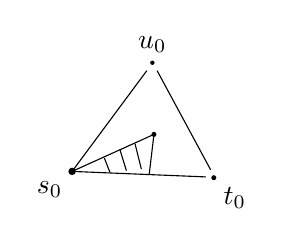
\begin{tikzpicture}[x=1cm,y=1cm,baseline]
\coordinate (s) at (0,0); \coordinate (t) at (1.8,-.08); \coordinate (u) at (1.02,1.38);
\draw (s)--(.95,1.28) (1.08,1.28)--(1.76,.02) (1.7,-.07)--(s);
\draw (s)--(1.04,.47)--(.98,-.035);
\draw (.41,.17)--(.48,-.01) (.61,.27)--(.69,.01) (.8,.35)--(.88,.03);
\fill (s) circle (.047) (t) circle (.032) (u) circle (.028) (1.04,.47) circle (.032);
\node[below left] at (s) {$s_0$}; \node[below right] at (t) {$t_0$}; \node[above] at (u) {$u_0$};
\end{tikzpicture}}

(p.ex. $\rho={}$``rotation d'un cran autour de $u_0$, de $s_0$ vers $t_0$''), on aura

% slanted
\margin{plus \unsure{joliment} : $\rho=\rho_1={}$ symétrie p.r. au centre de l'arête $\{s_0,t_0\}$, p. ex., ou $\rho=\rho_\infty$ (rotation de \unsure{un|$-1$} tiers de tour autour du centre de la face $\{s_0,t_0,u_0\}$\unsure{)}}

\[
\lambda^{-1}t_0=\lambda^{-1}\rho s_0=\rho\lambda^{-1}s_0
\]

posons

\[
\left.\begin{aligned}\lambda^{\deleted{\unsure{-1|1}}}s_0&=g.s_0\\
\lambda^{-1}s_0&=g^{-1}.s_0\end{aligned}\quad\right|\quad
\text{où }g\in\operatorname{Norm}_{G_0^+}(G^+_{0\,s_0})
\]

la relation (32 bis) s'écrit aussi

\[
\{g.s_0,\rho g^{-1}\deleted{\unsure{t}}s_0\}\in A_0
\]

ou encore

\[
\exists u\in G_0^+,\quad\text{avec }\ u(s_0,t_0)=(gs_0,\rho g^{-1}t_0)
\]

ou encore, écrivant $t_0=\rho s_0$

\[
u.s_0=g.s_0 \qquad u\rho.s_0=\rho g^{-1}.\deleted{\unsure{t}}s_0
\]

soit encore

\[
g^{-1}u\in G^+_{0\,s_0},g(\underbrace{\rho^{-1}u\rho})\in G^+_{0\,s_0}
\]

donc l'axiome $\mathrm T_0\,3$ équivaut :

% slanted
\margin{on a posé $g^{-1}u=z$ i.e. $u=gz$}

\[
\begin{aligned}
(\mathrm T_0\,3')\quad &\forall g\in\operatorname{Norm}_{G_0^+}(G^+_{0\,s_0}),\ \exists z\in G^+_{0\,s_0}\quad\text{(néc$^{\rm t}$ unique!)}\\
&\text{tel qu'on ait}\\
&g.\deleted{\unsure{\rho^{-1}|\rho}}\operatorname{int}(\rho^{-1})(gz)\in G^+_{0\,s_0}
\end{aligned}\tag*{(34)}
\]

% slanted
\margin{où $\rho$ est \deleted{\unsure{l'unique|l'antique}} \inserted{un} élément de $G_0^+$ fixé \deleted{\unsure{une}} fois pour toutes, tel que $\rho s_0=t_0$, NB \unsure{la|$\rho$}, $\rho=\rho_1$ ou $\rho=\rho_\infty$}

Si on se rappelle que la situation d'un 2-polyèdre orienté \inserted{triangulé} régulier \deleted{\unsure{avec|com.|comme}}, spécifié par $(s_0,t_0,u_0)$, équivaut : celle du groupe $G_0^+$, avec des
% archive sheet number: 111
